\documentclass{article}[11pt]
%-----------Packeges---------------%
\usepackage{amsmath}
\usepackage{amssymb}
\usepackage{amsfonts}
\usepackage{tocloft}
\usepackage{float}
\usepackage{graphicx}
\usepackage[bookmarks=true]{hyperref}
\usepackage{fancyhdr}


%----------Definition & Theorem----%
\newtheorem{definition}{Definition}[subsection]
\newtheorem{theorem}{Theorem}[subsection]
\newtheorem{proposition}{Proposition}[subsection]
\newtheorem{lemma}{Lemma}[subsection]
\newtheorem{corollary}{Corollary}[subsection]

\pagestyle{fancy}
\fancyhead[L]{Math 461}
\fancyhead[C]{HW2}
\fancyhead[R]{Lanxiao Bai(lbai5)}
\begin{document}
	\paragraph{0.1}\textbf{Solution:}
		\subparagraph{(a)} \[n = (2 \times 3)^{15} = 470184984576\]
		\subparagraph{(b)} \[n = (2 \times 3)^{14} \times 15 \times 3 = 3526387384320\]
		\subparagraph{(c)} \[(2 \times 2)^{15} = 1073741824\]
	\paragraph{0.2}\textbf{Solution:}
		\subparagraph{(a)} \[P(A^S \cap B^S) = 1 - 0.3 -0.5 = 0.2\]
		\subparagraph{(b)} \[P(A \cap B^S) = P(A) = 0.3\]
		\subparagraph{(c)} \[P(A \cap B) = P(\emptyset) = 0\]
	\paragraph{0.3}\textbf{Solution:} 
	\begin{align}
		&P(Accept) = P(American\ Express) + P(Visa) - P(American\ Express) \cap P(Visa)\nonumber\\
		&\phantom{P(Accept)} = 0.24 + 0.61 - 0.11\nonumber\\
		&\phantom{P(Accept)} = 0.74\nonumber
	\end{align}
	\paragraph{0.4}\textbf{Solution:} \[P(Blackjack) = \frac{4 \times 16}{\binom{52}{2}} = \frac{64}{1326} = 0.048\]
	\paragraph{0.5}\textbf{Solution:} 
	\begin{align}
		&P(No\ blackjack) = 1 - P(I \cup Dealer)\nonumber\\
		&\phantom{P(No\ blackjack)} = 1 - (P(I) + P(Dealer) - P(I) \cap P(Dealer))\nonumber\\
		&\phantom{P(No\ blackjack)} = 1 - (0.048 + 0.048 - \frac{2(4 \times 16)(3 \times 15)}{\binom{52}{4}})\nonumber\\
		&\phantom{P(No\ blackjack)} = 1 - (0.096 - 5760/270725) = 1 - 0.075 = 0.925\nonumber
	\end{align}
	\paragraph{0.6}\textbf{Solution:} 
		\subparagraph{(a)}
		\begin{align}
			&P(1) = 4/20 = 0.2\nonumber\\
			&P(2) = 8/20 = 0.4\nonumber\\
			&P(3) = 5/20 = 0.25\nonumber\\
			&P(4) = 2/20 = 0.1\nonumber\\
			&P(5) = 1/20 = 0.05\nonumber
		\end{align}
		\subparagraph{(b)}
		\begin{align}
			&n = 4 \times 1 + 8 \times 2 + 5 \times 3 + 2 \times 4 + 5 = 48\nonumber\\
			&P(1) = 4/48 = 1/12\nonumber\\
			&P(2) = 16/48 = 1/3\nonumber\\
			&P(3) = 15/48 = 5/16\nonumber\\
			&P(4) = 8/48 = 1/6\nonumber\\
			&P(5) = 5/48\nonumber
		\end{align}
	\paragraph{0.7}\textbf{Solution:} In a single roll, 
	\begin{align}
		&P(5) = 4/36 = 1/9\nonumber\\
		&P(7) = 6/36 = 1/6\nonumber\\
		&P(5 \cup 7) = 10/36 = 5/18\nonumber\\
		&P(not\ 5\ and\ not\ 7) = 1 - 5/18 = 13/15\nonumber
	\end{align}
		Thus,
			\[P(E_n) = (13/15)^{n-1}/9\]
		and
			\[P(5\ comes\ first) = \sum_{n=1}^\infty P(E_n) = \lim_{n\rightarrow \infty} \frac{5}{6}[1 - (\frac{13}{15})^{n}] = \frac{5}{6}\]
	\paragraph{0.8}\textbf{Solution: }In a single draw,
	    \[P(red) = 3/10\]
	    \[P(black) = 7/10\]
	    If denote the event that A will draw the first red ball in the nth cycle as $E_n$,
	    \begin{align}
	    &P(E_n) = \frac{3}{10 - 2(n-1)} \prod_{i = 1}^{n-1} (\frac{9 - 2n}{12 - 2n} \frac{8 - 2n}{11 - 2n} \nonumber\\
	    &\phantom{P(E_n)} = \frac{3}{12 - 2n} \prod_{i = 1}^{n-1} (\frac{9 - 2n}{12 - 2n} \frac{8 - 2n}{11 - 2n})\nonumber
	    \end{align}
	    Since there are only 7 black balls, so A can only draw red ball in the first 4 cycles. Thus,
	    \[P(A) = \sum_{i = 1}^4 P(E_n) = 3/10 + 7/40 + 1/12 + 1/40  = 7/12\]
	\paragraph{0.9}\textbf{Solution:}
	    \subparagraph{(a)} \[P(same) = P(red) + P(green) + P(blue) = (5/19)^3 + (6/19)^3 + (8/19)^3 = 0.124\]
	    \subparagraph{(b)} \[P(diff) = (5/19)(6/19)(8/19) = 0.035\]
	\paragraph{0.10}\textbf{Solution:} Having a girl on position i means to randomly choose a girl to interlope her into the rest $b + g - 1$ people to divide any permutation of them into 2 part. Thus,
	\[P(i) = \frac{(b + g - 1)!g}{(b + g)!} = \frac{g}{b + g}\]
	\paragraph{0.11}\textbf{Proof:} $EF^C = (E^C)^CF^C = (E^C \cup F)^C$, then $P(EF^C) = P((E^C \cup F)^C) = 1 - P(E^C \cup F) = 1 - (P(E^C) + P(F) - P(E^CF)) = 1 - ((1 - P(E)) + P(F) - P(E^CF)) = 1 - 1 + P(E) - P(F) + P(E^CF) = P(E) - (P(F) - P(E^CF)) = P(E) - P(EF)\blacksquare$
	\paragraph{0.12}\textbf{Proof:} $P(EF) = P((E^C)^C(F^C)^C) = P((E^C \cup F^C)^C) = 1 - P((E^C \cup F^C)) = 1 - (P(E^C) + P(F^C) - P(E^CF^C)) = 1 - ((1 - P(E)) + (1 - P(F) - P(E^CF^C))) = 1 - (2 - (P(E) + P(F) - P(E^CF^C))) = (P(E) + P(F)) - 1 + P(E^CF^C) \geq P(E) + P(F) - 1\blacksquare$
	
		Base case is proved above, we can suppose that when $n = k$
		 \[P(\bigcap_{i = 1}^k E_i) \geq \sum_{i = 1}^k P(E_i) - (k - 1)\]
		 is true.
		 
		 When $n = k + 1$, 
		 \begin{align}
		 	&P(\bigcap_{i = 1}^{k + 1} E_i) = P(\bigcap_{i = 1}^{k} E_i \cap E_{k + 1})\nonumber\\
		 	&\phantom{P(\bigcap_{i = 1}^{k + 1} E_i)} = P(((\bigcap_{i = 1}^{k} E_i)^C)^C \cap (E_{k + 1}^C)^C)\nonumber\\
		 	&\phantom{P(\bigcap_{i = 1}^{k + 1} E_i)} = P(((\bigcap_{i = 1}^{k} E_i)^C) \cup E_{k + 1}^C)^C)\nonumber\\
		 	&\phantom{P(\bigcap_{i = 1}^{k + 1} E_i)} = 1 - P((\bigcap_{i = 1}^{k} E_i)^C \cup E_{k + 1}^C)\nonumber\\
		 	&\phantom{P(\bigcap_{i = 1}^{k + 1} E_i)} = 1 - (P((\bigcap_{i = 1}^{k} E_i)^C) + P(E_{k + 1}^C) - P((\bigcap_{i = 1}^{k} E_i)^CE_{k + 1}^C)\nonumber\\
		 	&\phantom{P(\bigcap_{i = 1}^{k + 1} E_i)} = 1 + P((\bigcap_{i = 1}^{k} E_i)^CE_{k + 1}^C) - ((1 - P(\bigcap_{i = 1}^{k} E_i)) + (1 - P(E_{k + 1})))\nonumber\\
		 	&\phantom{P(\bigcap_{i = 1}^{k + 1} E_i)} = P((\bigcap_{i = 1}^{k} E_i)^CE_{k + 1}^C) + P(\bigcap_{i = 1}^{k} E_i) + P(E_{k+1}) - 1\nonumber
		 \end{align}
		 
		 According to our hypothesis
		 \[
		 	P(\bigcap_{i = 1}^k E_i) \geq \sum_{i = 1}^k P(E_i) - (n - 1)\nonumber
		 \]
		 Then
		 \begin{align}
		 	&P(\bigcap_{i = 1}^{k+1} E_i) \geq \sum_{i = 1}^k P(E_i) - (n - 1) + P(E_{k+1}) - 1\nonumber\\
		 	&\phantom{P(\bigcap_{i = 1}^{k+1} E_i)} \geq \sum_{i = 1}^k P(E_i) - (n - 1) + P(E_{k+1}) - 1\nonumber\\
		 	&\phantom{P(\bigcap_{i = 1}^{k+1} E_i)} \geq \sum_{i = 1}^{k + 1} P(E_i) - n\nonumber
		 \end{align}
		 We can conclude that $\forall n \in \mathbb{N}$
		 \[P(\bigcap_{i = 1}^n E_i) \geq \sum_{i = 1}^n P(E_i) - (n - 1)\]
		 $\blacksquare$
	\paragraph{0.13}\textbf{Solution:}
	\begin{figure}[H]
        \begin{center}
        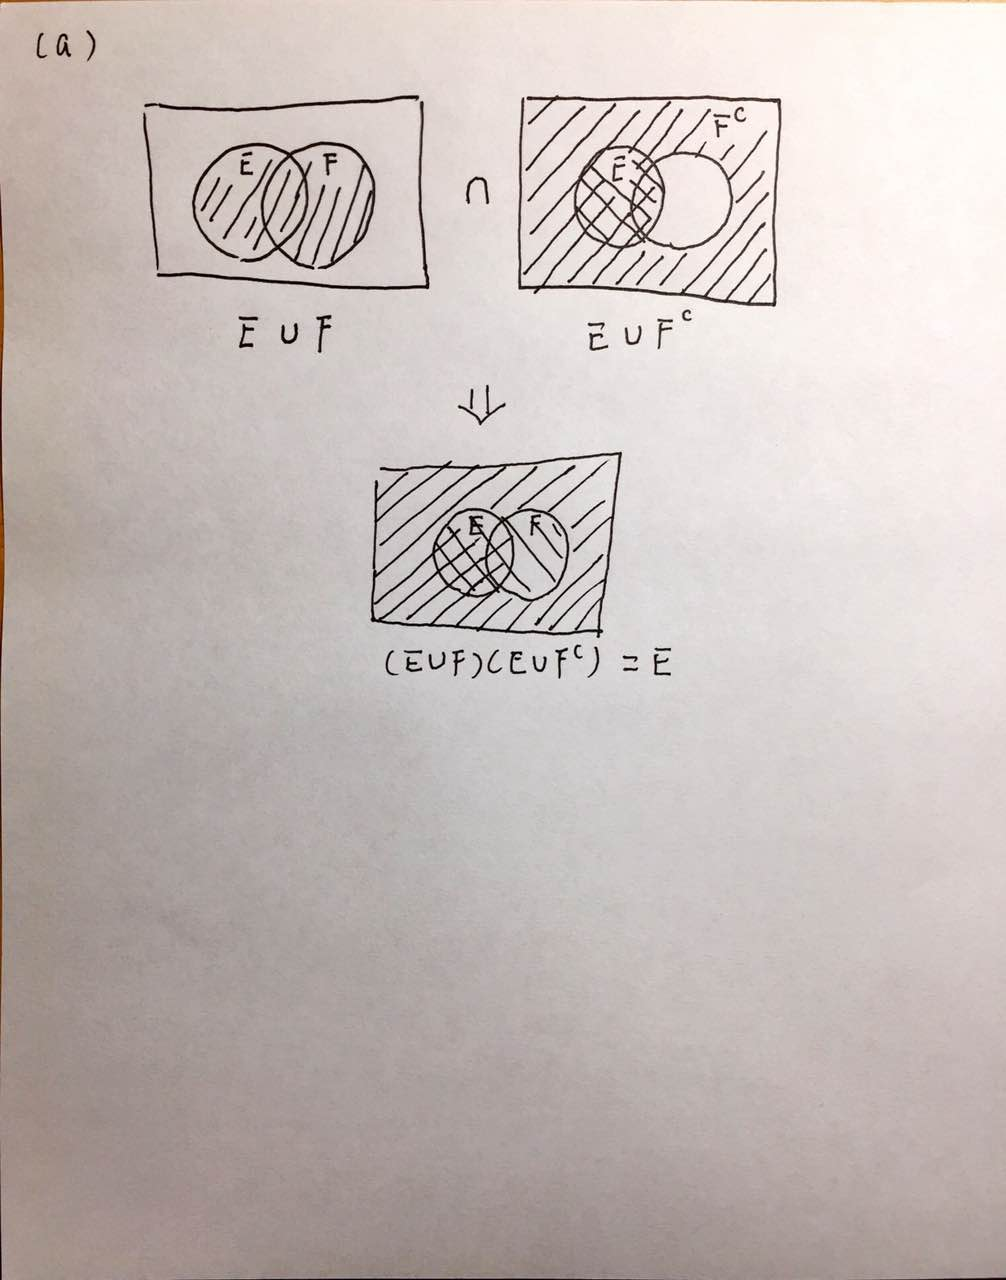
\includegraphics[width=10cm]{./imgs/2-13a.jpg}
        \caption{0.13.a}
        \end{center}
    \end{figure}
    \begin{figure}[H]
        \begin{center}
        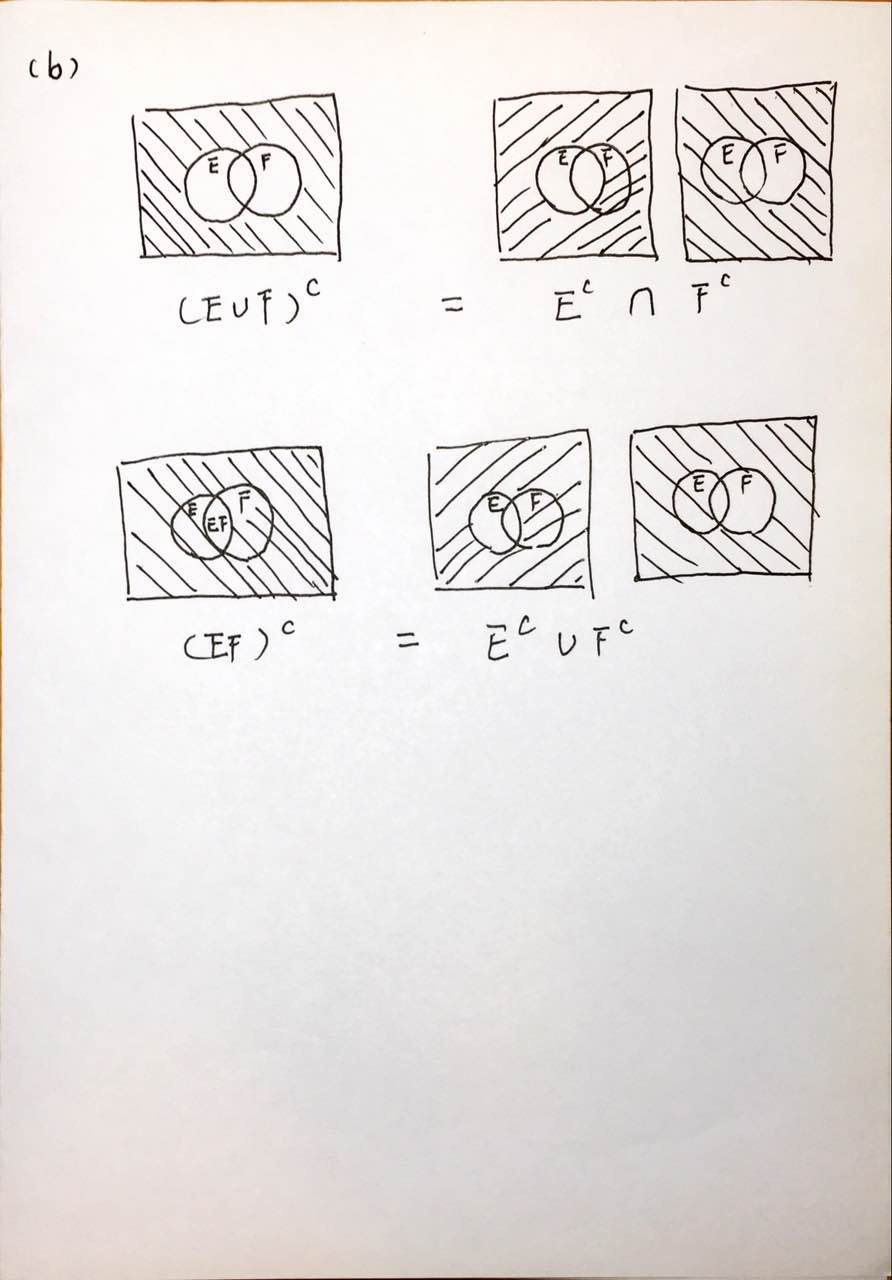
\includegraphics[width=10cm]{./imgs/2-13b.jpg}
        \caption{0.13.b}
        \end{center}
    \end{figure}
\end{document}